\documentclass[../main.tex]{subfiles}
\graphicspath{{\subfix{../figures/}}}
\begin{document}

\section{Cross Section Measurement}
\label{sec:xsec}
In a single differential cross section analysis, the dependence of the cross section on a specific variable is assessed.  The measured cross section in true bin $i$ of variable $X$ is
\begin{equation}
    \label{eq:xsec}
    \odv{\sigma}{X}_{i}^{} = \sum_{j} \frac{U_{ij} (N_{j} - B_{j})}{\Phi \ \epsilon_{i} \ N_{target}} \frac{1}{\Delta X_{i}},
\end{equation}
where $j$ is a reconstructed bin, and $N_{j}$, $B_{j}$, and $\epsilon_{j}$ are the number of selected events, the number of background events, and the selection efficiency in bin $j$, respectively.  $X_{i}$ is the true bin width, while $U_{ij}$ is an unfolding matrix that transofrms the background subtracted selected events in bin $j$ to bin $i$.  $\Phi$ is the integrated neutrino flux and $N_{target}$ is the number of argon targets in the fiducial volume, both of which are discussed in the following subsection.

\subsection{Input Preparation}

\subsubsection{Integrated Flux}
The simulated BNB muon neutrino flux at the center of the ICARUS detector, scaled to the unblinded Run 2 POT, is shown in Figure \ref{fig:icarusbnbfluxspectrum}.  From this, the integrated neutrino flux through the face of the fiducial volume for unblinded Run 2 data is taken to be
\begin{equation}
    \Phi = 8.25 \times 10^{09} \ \text{cm}^{-2}
\end{equation}

\begin{figure}[H]
    \center
    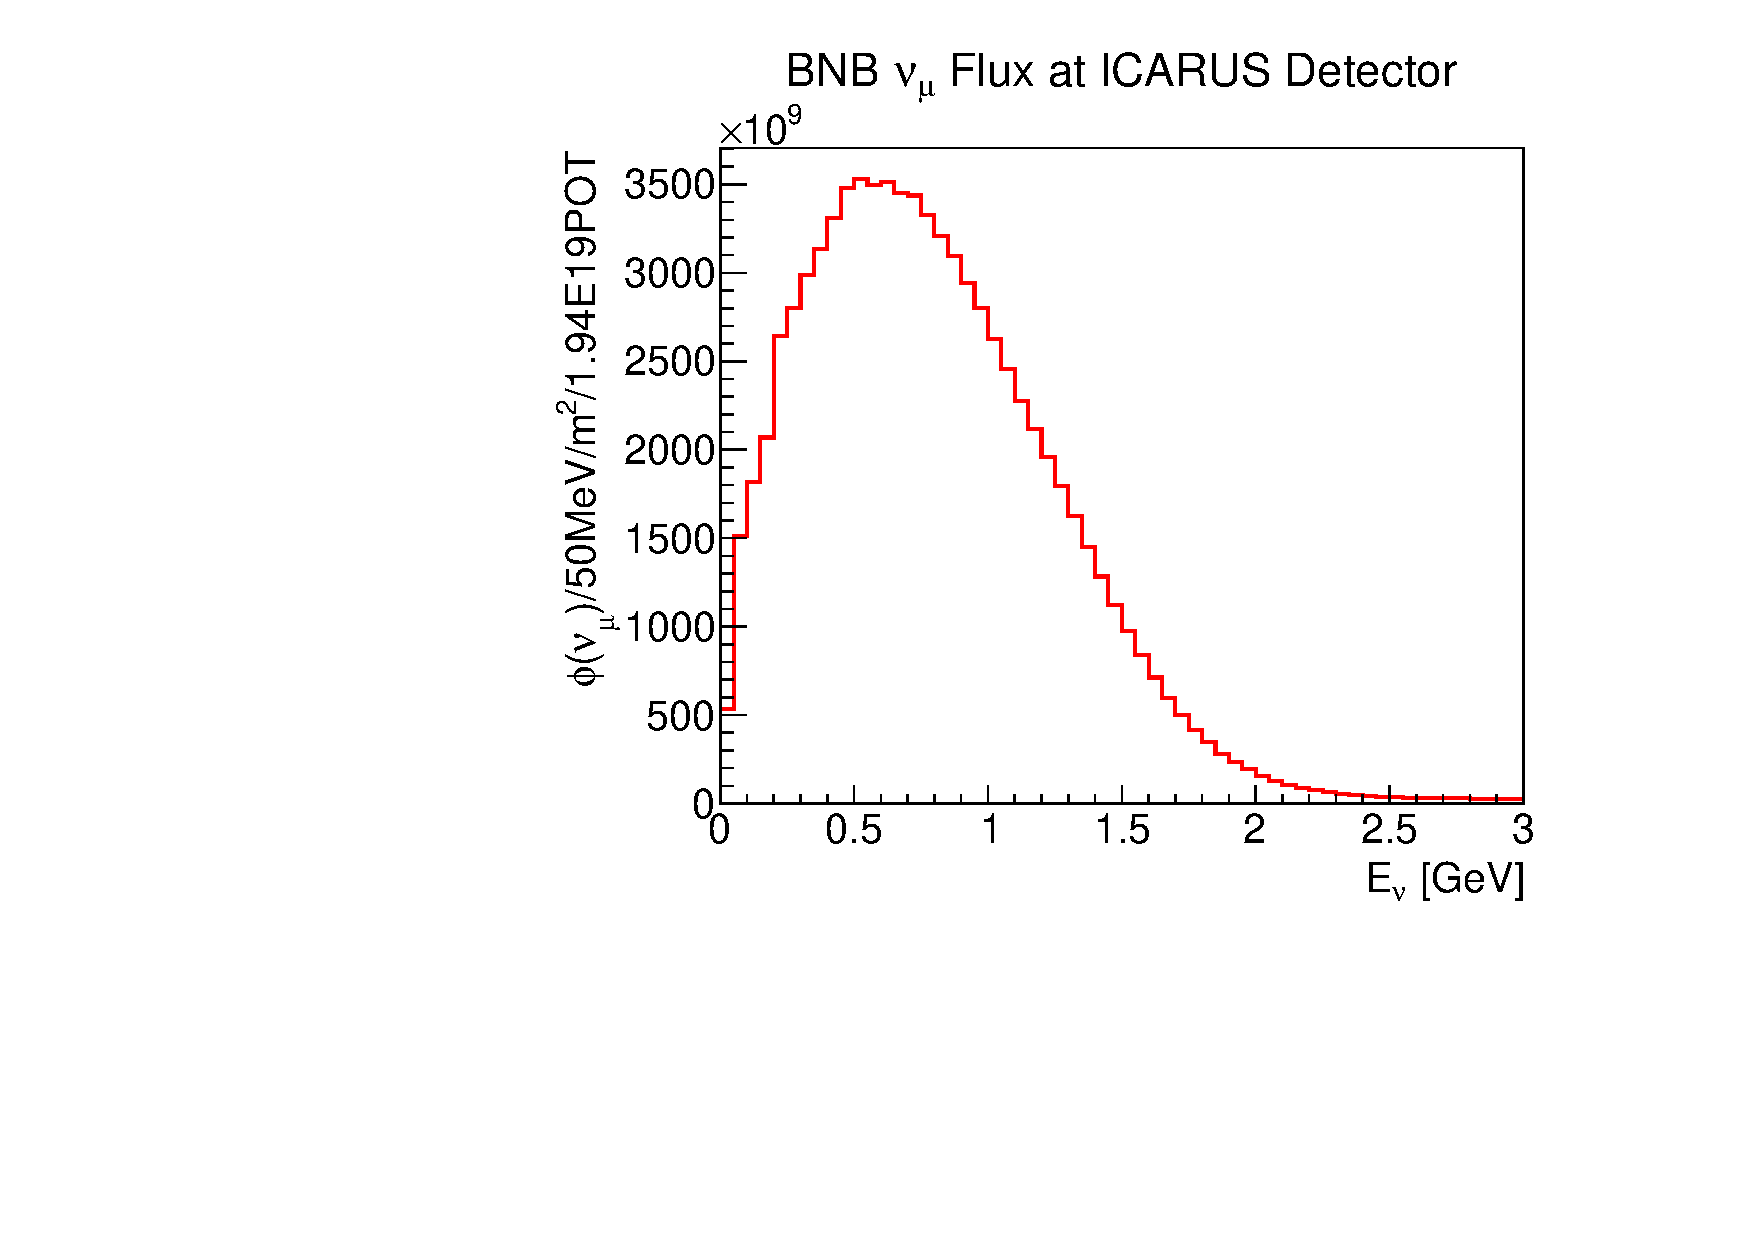
\includegraphics[width=0.90\textwidth]{icarusbnbfluxspectrum.pdf}
    \caption[text]{Muon neutrino flux at the ICARUS detector center, scaled to Run 2 unblinded POT.}
    \label{fig:icarusbnbfluxspectrum}
\end{figure}

\subsubsection{Number of Targets}
The number of fiducial nuclear argon targets, or $N_{target}$, is determined from the density of liquid argon $\rho$, the fiducial volume $V_{fiducial}$, and the atomic weight of argon $M_{Ar}$, and the number of nucleons per argon atom $N_{nucleons}$.
\begin{align}
\begin{split}
    N_{target} &= \frac{\rho \cdot V_{fiducial} \cdot N_{nucleons}}{M_{Ar}} \\
    &= \frac{1.39 [\frac{\text{g}}{\text{cm}^{3}}] \cdot 2.25 \times 10^{8} [\text{cm}^{3}] \cdot 40}{6.63 \times 10^{-23} [\text{g}]} \\
    &= 1.88 \times 10^{32} \ \text{nucleons}
\end{split}
\end{align}

\subsection{Cross Section Extraction Procedure}
Cross section measurements are carried out with the liklihood fitting and cross section extraction tool GUNDAM.  As an open-source framework, GUNDAM was first designed for T2K analyses and has since been used for NuMI cross section measurements at ICARUS.  This analysis marks the first use of GUNDAM in a BNB analysis.

To extract a cross section, the numerator of Equation \eqref{eq:xsec}, or the number of background-subtracted signal events for a given analysis bin after correcting for detector smearing, is first computed.  This is achieved through binned liklihood fitting, where template parameters controlling the number of Monte Carlo signal events in each analysis bin are varied such that the number of reconstructed Monte Carlo events best match observed counts from data.  Nuissance parameters corresponding to flux, interaction, and detector systematic uncertainties are simultaneously considered in the fit.

After determining the number of signal events from the fit, Equation \eqref{eq:xsec} is used to compute the differential cross section.  To propagate uncertainty of the fit to the final cross section result, many universes are created in which best-fit parameters are varied within the uncertainties allowed by the post-fit covariance matrix.  The cross section is recalculated for each universe, and the total uncertainty on the measurement is taken as the standard deviation across all universes.

\subsection{Asimov Extraction}
To demonstrate the GUNDAM cross section extraction machinery is functional and compatible with SPINE reconstructed output, an Asimov study in which selected event counts in data are assumed to be equal to those from Monte Carlo is carried out.  Results are shown in Figure \ref{fig:xsec_var_results_asimov}, and comparisons to the neutrino generator prediction will be made in Section \ref{subsec:xsec_validation}.

\begin{figure}[H]
    \center
    \subfloat[Muon momentum]
        {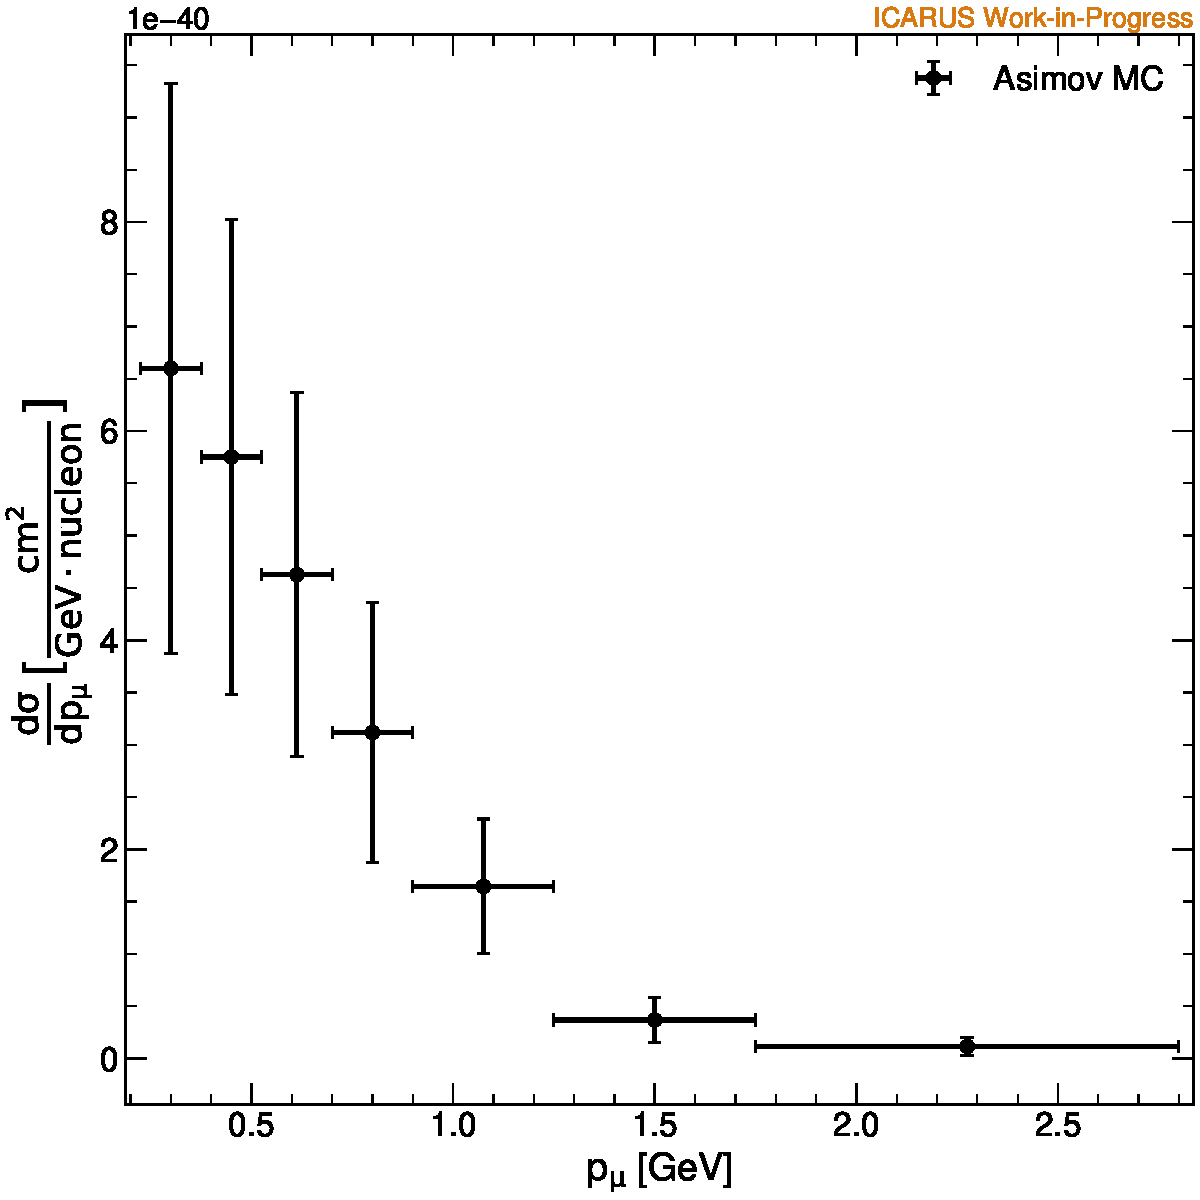
\includegraphics[width=0.50\textwidth]{xsec_muon_momentum_mag_asimov.pdf} \label{subfig:muon_momentum_mag_xsec_asimov}}
    \subfloat[Muon angle with respect to neutrino beam]
        {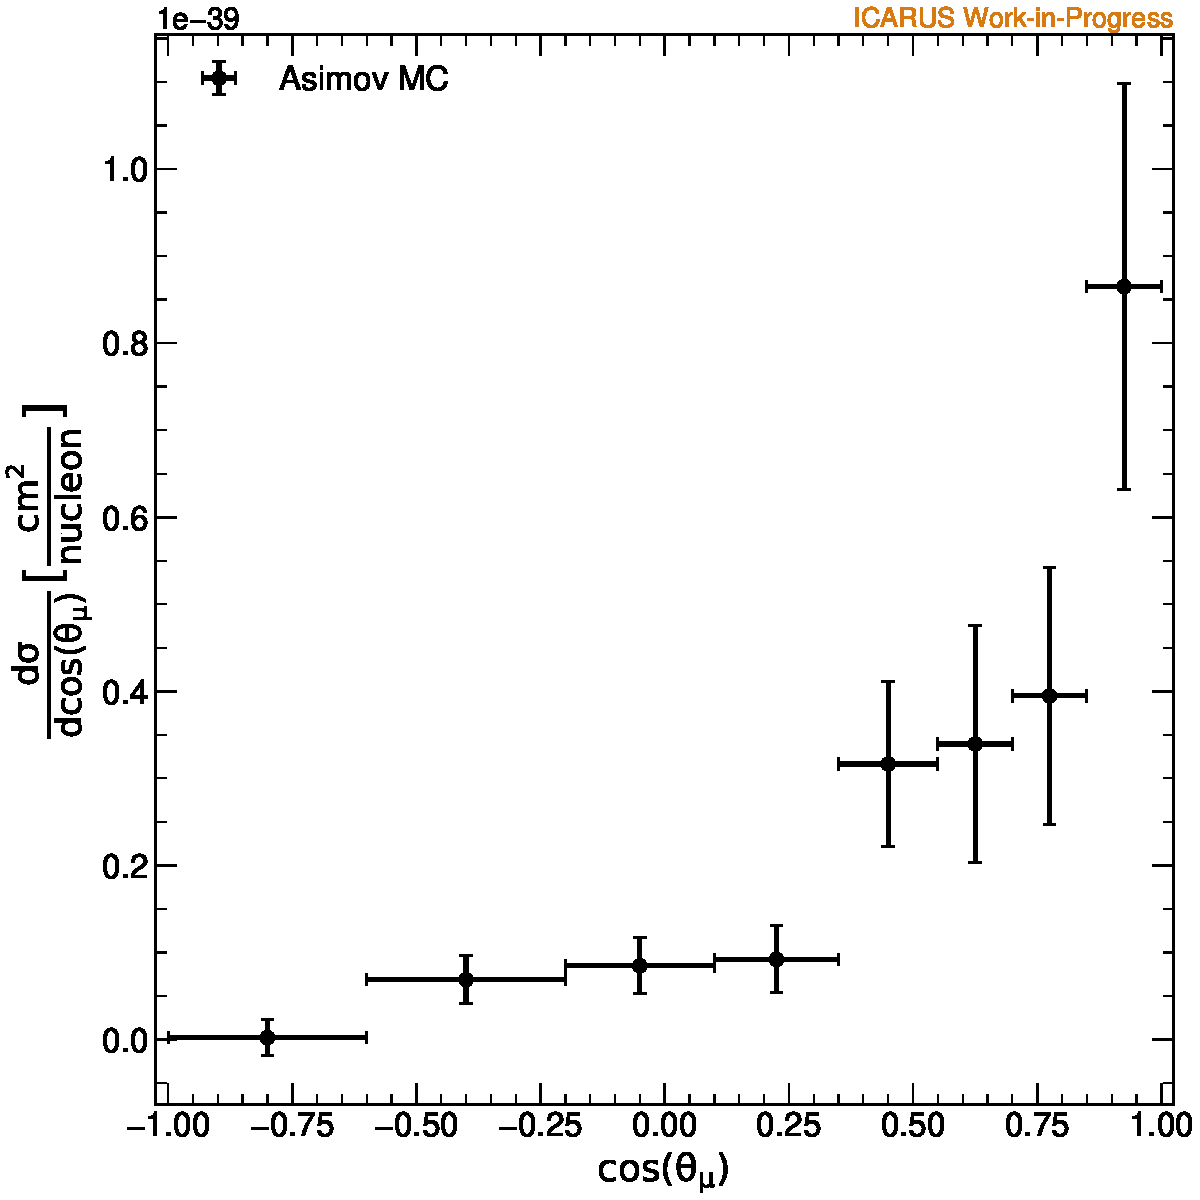
\includegraphics[width=0.50\textwidth]{xsec_muon_beam_costheta_asimov.pdf} \label{subfig:muon_beam_costheta_xsec_asimov}} \\
    \subfloat[Neutral pion momentum]
        {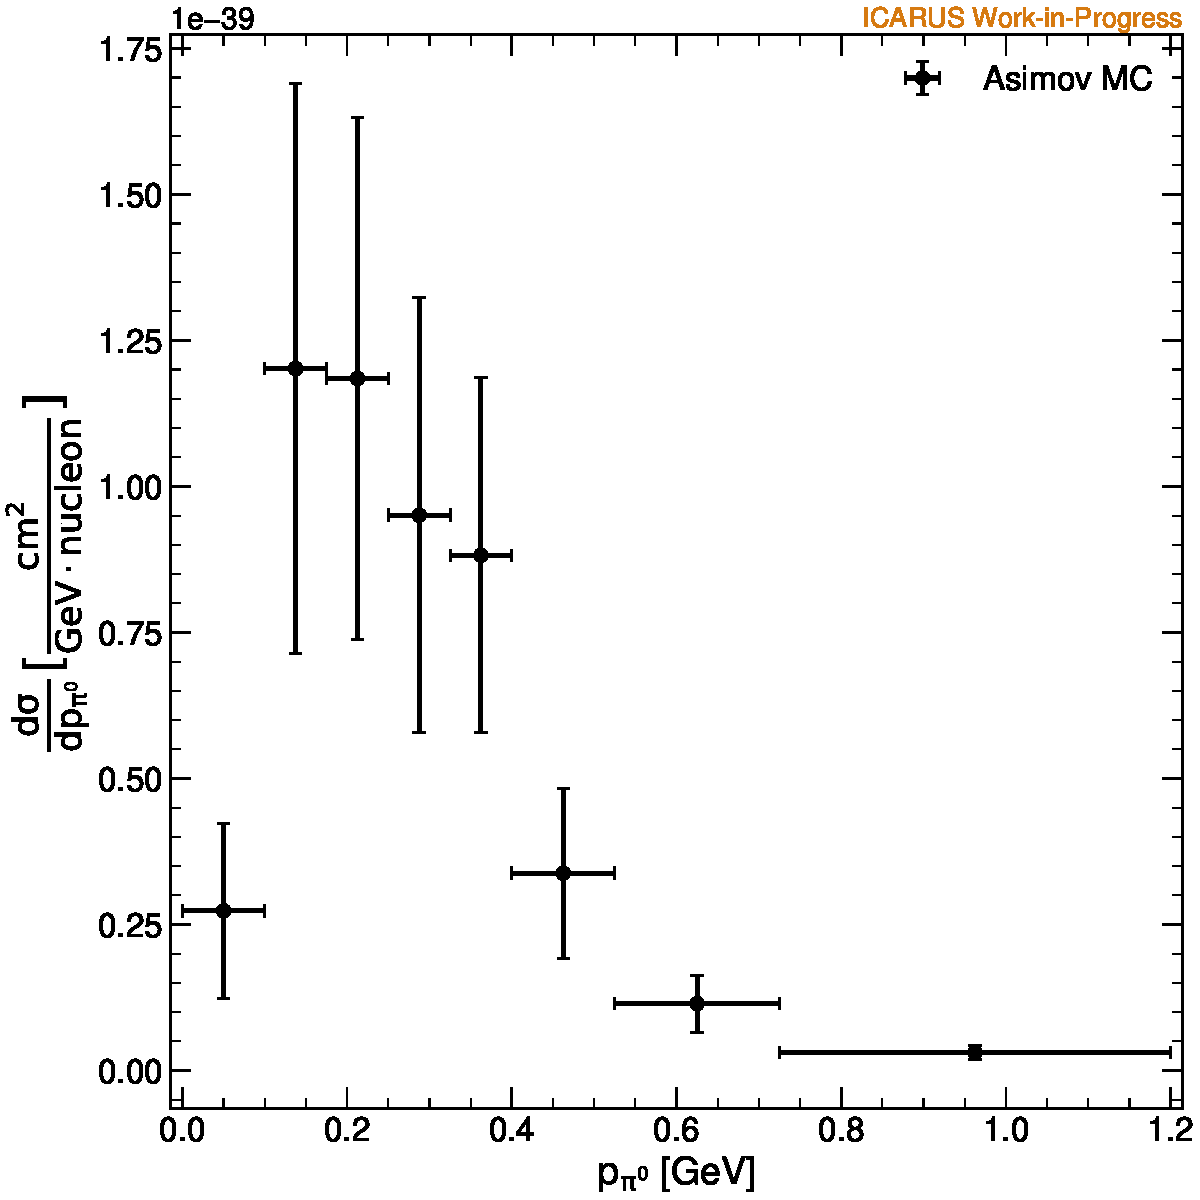
\includegraphics[width=0.50\textwidth]{xsec_pi0_momentum_mag_asimov.pdf} \label{subfig:pi0_momentum_mag_xsec_asimov}}   
    \subfloat[Neutral pion angle to neutrino beam]
        {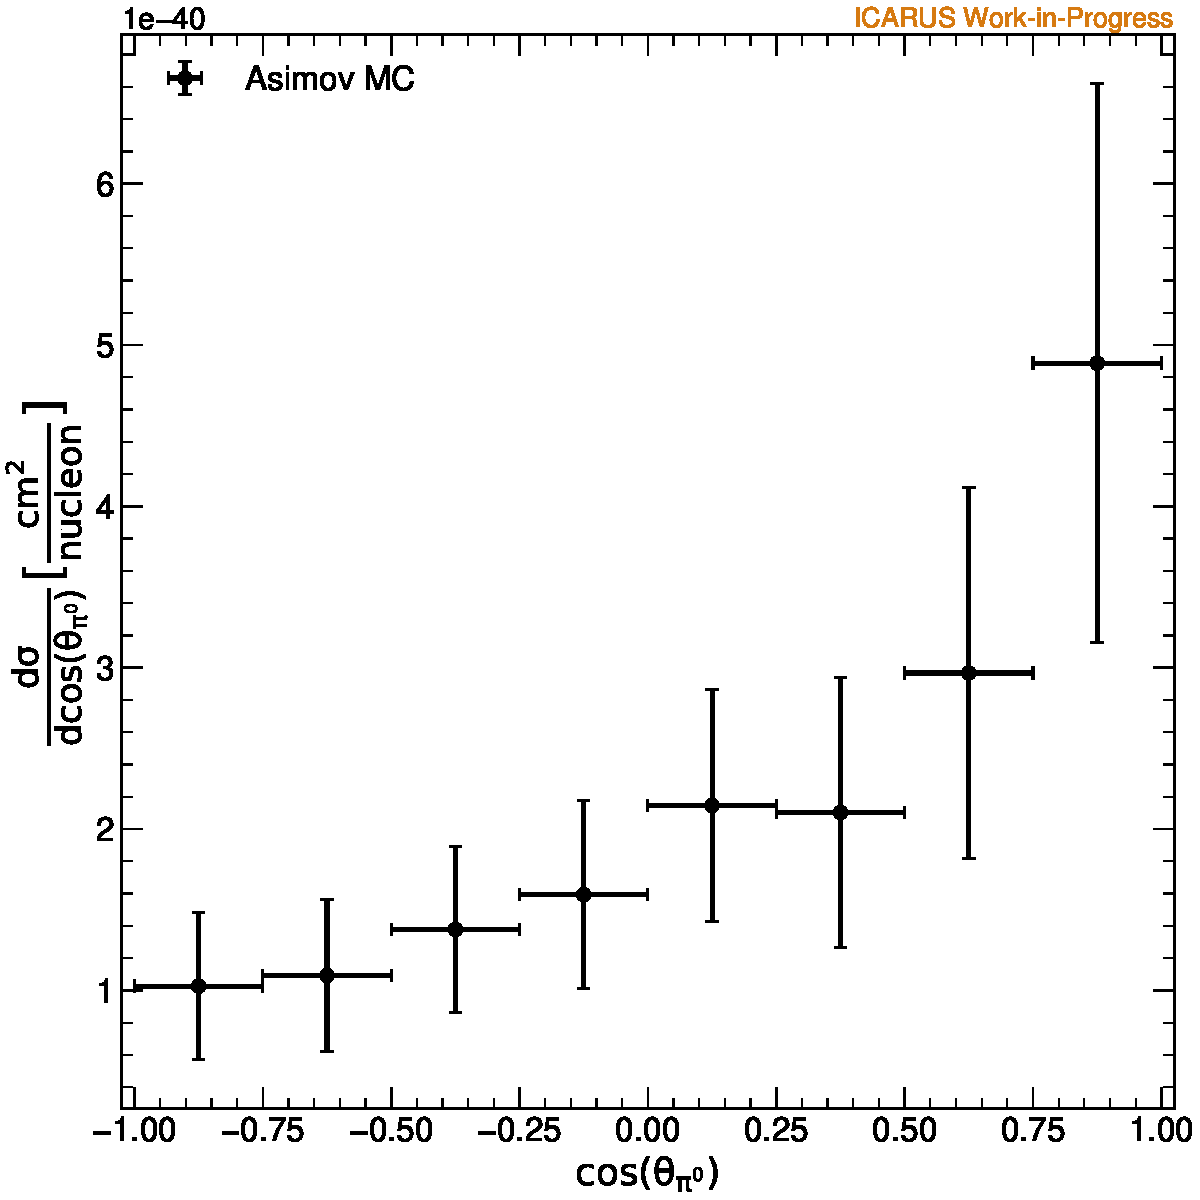
\includegraphics[width=0.50\textwidth]{xsec_pi0_beam_costheta_asimov.pdf} \label{subfig:pi0_beam_costheta_xsec_asimov}}          
    \caption{Asimov cross section extraction for for analysis variables}
    \label{fig:xsec_var_results_asimov}
\end{figure}

\subsection{Validation}
\label{subsec:xsec_validation}
\textcolor{red}{To-do: Include closure tests, p-value tests, etc.}

\subsection{Results}

\end{document}